\chapter{Introduzione generale}

\section{Principi generali}
Il problema della determinazione della pressione barometrica dell'atmosfera di Giove non ha ricevuto finora una soluzione soddisfacente, per l'elementare motivo che il pianeta suddetto si trova ad una distanza tale che i mezzi attuali non consentono di eseguire una misura diretta.
La \gls{api} è un componente essenziale per lo sviluppo del software.
\acrlong{gcd}
Conoscendo per\`o con grande precisione le orbite dei satelliti principali di Giove, e segnatamente le orbite dei satelliti medicei, \`e possibile eseguire delle misure indirette, che fanno ricorso alla nota formula \cite{gal}:
\begin{equation} \label{eq:eq1}
\Phi = K\frac{\Xi^2 +\Psi_\mathrm{max}}{1+\gei\Omega}\ .
\end{equation}

In \eqref{eq:eq1} le varie grandezze hanno i seguenti significati:
\begin{enumerate}
\item $\Phi$ angolo di rivoluzione del satellite in radianti se $K=1$, in gradi se $K=180/\pi$;
\item $\Xi$ eccentricit\`a dell'orbita del satellite; questa \`e una grandezza priva di dimensioni;
\item $\Psi_\mathrm{max}$ rapporto fra il semiasse maggiore ed il semiasse minore dell'orbita del satellite, nelle condizioni di massima eccentricit\`a;
\item $\Omega$ velocit\`a istantanea di rotazione; 
\end{enumerate}

Le grandezze in gioco sono evidenziate nella Figura \ref{fig:figura}.
\begin{figure}[htb]\centering
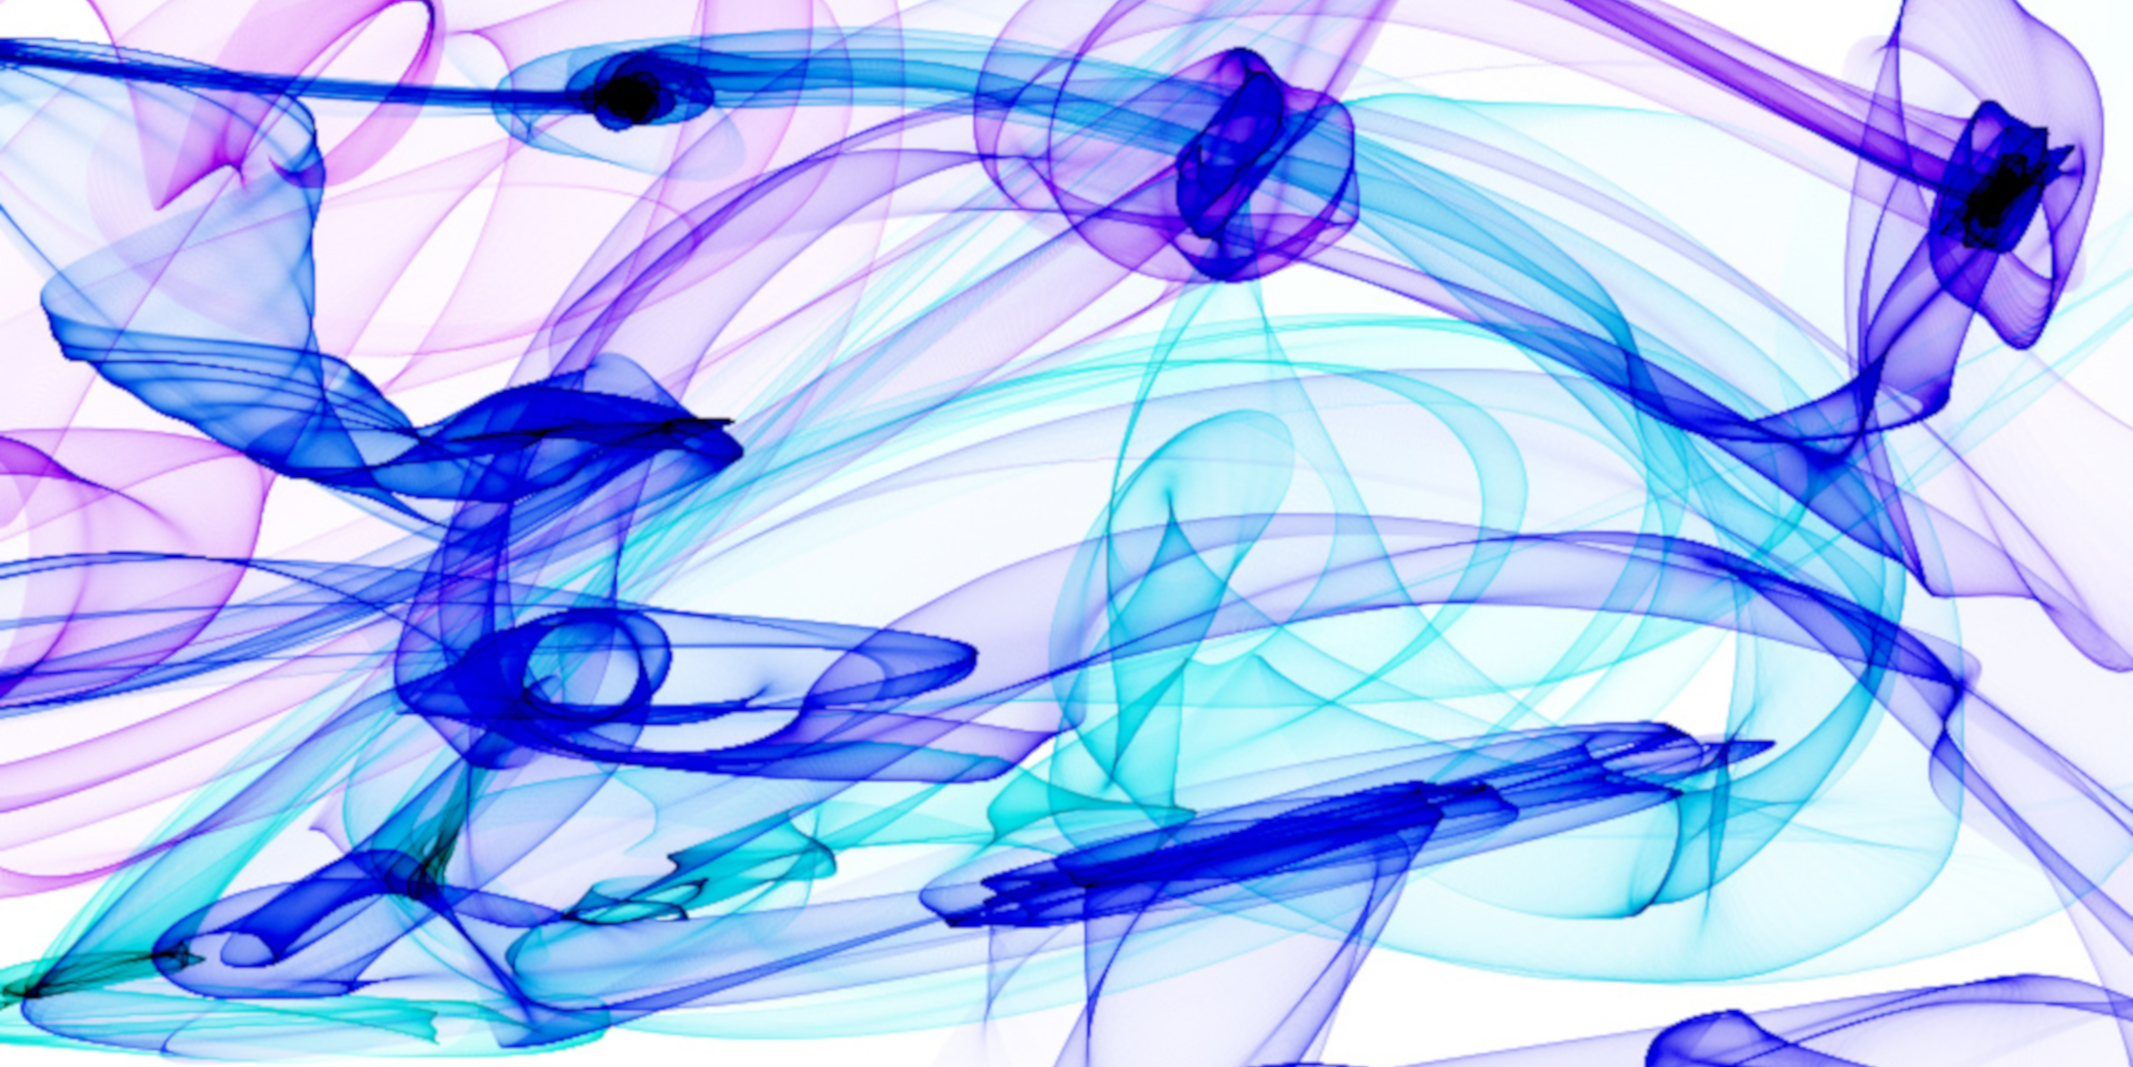
\includegraphics[scale=0.1]{./Images/FlameArtwork2.jpg}
\caption{Come includere una figura, salvata nella cartella immagini.}\label{fig:figura}
\end{figure}




\chapter{Il barometro}
\section{Generalit\`a}
In questa sezione proviamo a modificare l'INTERLINEA.\\

\begin{interlinea}{0.87}
Il barometro, come dice il nome, serve per misurare la pesantezza; pi\`u precisamente la pesantezza dell'aria riferita all'unit\`a di superficie.
\end{interlinea}

\begin{interlinea}{2}
Studiando il fenomeno fisico si pu\`o concludere che in un dato punto grava il peso della colonna d'aria che lo sovrasta, e che tale colonna \`e tanto pi\`u grave quanto maggiore \`e la superficie della sua base; il rapporto fra il peso e la base della colonna si chiama pressione e si misura in once toscane al cubito quadrato, \cite{tor1}; nel Ducato di Savoia la misura in once al piede quadrato \`e quasi uguale, perch\'e col\`a usano un piede molto grande, che \`e simile al nostro cubito.
\end{interlinea}

\subsection{Forma del barometro}
Il barometro consta di un tubo di vetro chiuso ad una estremit\`a e ripieno di mercurio, capovolto su di un vaso anch'esso ripieno di mercurio; mediante un'asta graduata si pu\`o misurare la distanza fra il menisco del mercurio dentro il tubo e la superficie del mercurio dentro il vaso; tale distanza \`e normalmente di 10 pollici toscani, \cite{tor1,tor2}, ma la misura pu\`o variare se si usano dei pollici diversi; \`e noto infatti che gl'huomini sogliono avere mani di diverse grandezze, talch\'e anche li pollici non sono egualmente lunghi.

\section{Del mercurio}
Il mercurio \`e un a sostanza che si presenta come un liquido, ma ha il colore del metallo. Esso \`e pesantissimo, tanto che un bicchiere, che se fosse pieno d'acqua, sarebbe assai leggiero, quando invece fosse ripieno di mercurio, sarebbe tanto pesante che con entrambe le mani esso necessiterebbe di essere levato in suso.


\setcounter{footnote}{25}

Il Monte Amiata, che \`e locato nel territorio del Ducato%
\footnote{Naturalmente stiamo parlando del Granducato di Toscana.%
\ifclassica\NoteWhiteLine\fi
} del nostro Eccellentissimo et Illustrissimo Signore Granduca di Toscana\footnote{Cosimo IV de' Medici.}, \`e uno dei luoghi della terra dove pu\`o rinvenirsi in gran copia un sale rosso, che nomasi \emph{cinabro}, dal quale con artifizi alchemici, si estrae il mercurio nella forma e nella consistenza che occorre per la costruzione del barometro terrestre%
\ifclassica
\nota{Nota senza numero\dots

\dots e che va a capo.
}\fi.

La densit\`a del mercurio \`e molto alta e varia con la temperatura come pu\`o desumersi dalla tabella \ref{t:1}.

\begin{table}[htp]              
\centering                      
\begin{tabular}%                
{r c l p{5cm}}                  % parametri di incolonnamento: r (a destra), c (al centro), l (a sinistra),
								% p (per definire la larghezza della colonna)
\hline\hline
Colonna 1 & Colonna 2 & Colonna 3 & Colonna 4 \\  
\hline
\hspace*{1.3em}
  & 10  & 100 & 13,8  \\
2 & 20  &     & 13,6  \\
  & 30  & 300 & 13,5  \\
4 & 40  &     & 13,3  \\
\hline \hline
\end{tabular}
\caption[Descrizione breve: compare nell'elenco tabelle]{Descrizione completa: didascalia della tabella.} \label{t:1}  
%[Short description for the content list.]{Complete descreption: caption of the table.}
\end{table}



\begin{table}[htp]              
\centering                      
\begin{tabular}{d d}                        
\hline\hline                    
\multicolumn{1}{c}{Temperatura} & \multicolumn{1}{c}{Densit\`a}  \\  
\multicolumn{1}{c}{\unit{\gradi C}} & \multicolumn{1}{c}{$\unit{t/m^3}$}  \\
\hline%                        
\hspace*{1.3em}
0 & 13.8 \\   
10 & 13.6 \\   
50 & 13.5 \\   
100 & 13.3 \\   
\hline \hline
\end{tabular}
\caption[Densit\`a del mercurio]{Densit\`a del mercurio. Si pu\`o fare molto meglio usando il pacchetto \textsf{booktabs}.} \label{t:2}  % didascalia con label
\end{table}



%
\begin{observation}\normalfont
This is the English version of \emph{Osservazione}.
\end{observation}

Per nostra fortuna, questo grande freddo, che necessita per la confetione de li sorbetti, molto raramente, se non mai, viene a formarsi nelle terre del Granduca Eccellentissimo, sicch\'e non vi ha tema che il barometro di mercurio possa essere ruinato dal grande gelo e non indichi la pressione giusta, come invece deve sempre fare uno strumento di misura, quale \`e quello che \`e descritto cost\`i \cite{duane1964}.


%%%%%%%%%%%%%%%%%%%%%%%%%%%%%%%%%%%%%%%%%%%%%%%%
%%%%%%%%%%%%%%%%%%%%%%%%%%%%%%%%%%%%%%%%%%%%%%%%

%This example is to show how to include .tex files


\chapter{Primo capitolo della seconda parte}

\section{How to}
Il testo di questo capitolo di trova in un file .tex separato!, nella cartella Part\_II

\lipsum[1]